\documentclass[14pt]{extarticle} 
\usepackage[T1,T2A]{fontenc}
\usepackage[utf8]{inputenc}
\usepackage[top=2.5cm,bottom=2.5cm,left=2.5cm,right=2.5cm]{geometry}
\usepackage[english,ukrainian]{babel}
\usepackage{indentfirst} % indents first par

\usepackage{graphicx}
\graphicspath{ {./images/} } % for inserting images 		\includegraphics[width=\textwidth]{pic0}
\usepackage{float} %\begin{figure}[H] to force image placement
\usepackage{amsfonts,amsmath,amsthm,amscd,amssymb,latexsym, mathtools}

\title{Data Analysis \\  Індивідуальне завдання 1}
\author{Бойченко Вікторія}
\date{}

\begin{document}

\maketitle

\section{ Завантажити данні в електронну таблицю. Скласти інтервальний статистичний ряд (таблицю частот). Кількість інтервалів групування – формула Стерджесса. (1)}

\begin{enumerate}

\item  Скопіювавши дані в ексель, обираємо відповідний варіант (№1)

\item Складаємо варіаційний ряд (за зростанням)

\item Скласти інтервальний статистичний ряд (таблицю частот)

\begin{enumerate}

\item Розмах вибірки:
\[ w = x_{max} - x_{min} = 0,843 - 0,081 = 0,762 \] 

\item Число інтервалів групування за формулою Стерджесса:
\[ k = 1 + \log_2{n} = 7,781 \approx 8 \] 

\item Довжина інтервалу групування:
\[ \Delta = \frac{w}{k} =  \frac{0,762}{8} = 0,09525 \approx 0,1\]

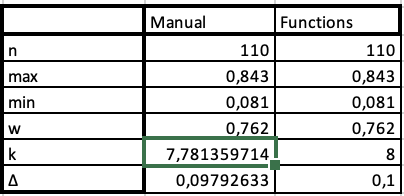
\includegraphics[width=\textwidth/2]{zvit1-start}


\item $x_i^* = a_{i-1} + \frac{\Delta}{2} \quad - $ середина і-го інтервалу, $i=\overline{1,k}$ 

де $a_{0} = x_{min} ,\; a_{k} = x_{max}$

\item $n_i^* $ - кількість значень, що потрапляли у відповідний інтервал

\item Формуємо згруповану вибірку:

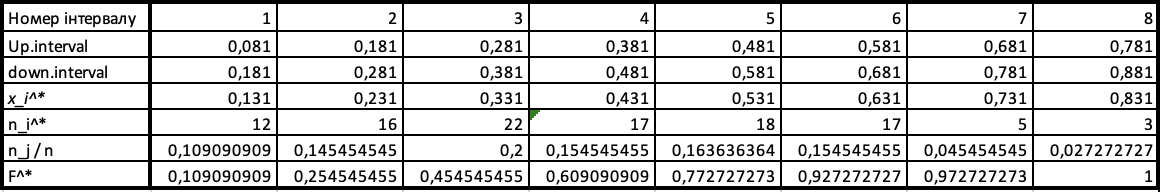
\includegraphics[width=\textwidth]{zvit1-0}

\end{enumerate}


\end{enumerate}

\section{Візуалізувати дані. Побудувати полігон, гістограму, емпіричну функцію розподілу, кумулятивну криву, відмітити на ній медіану та квартилі. (2)}

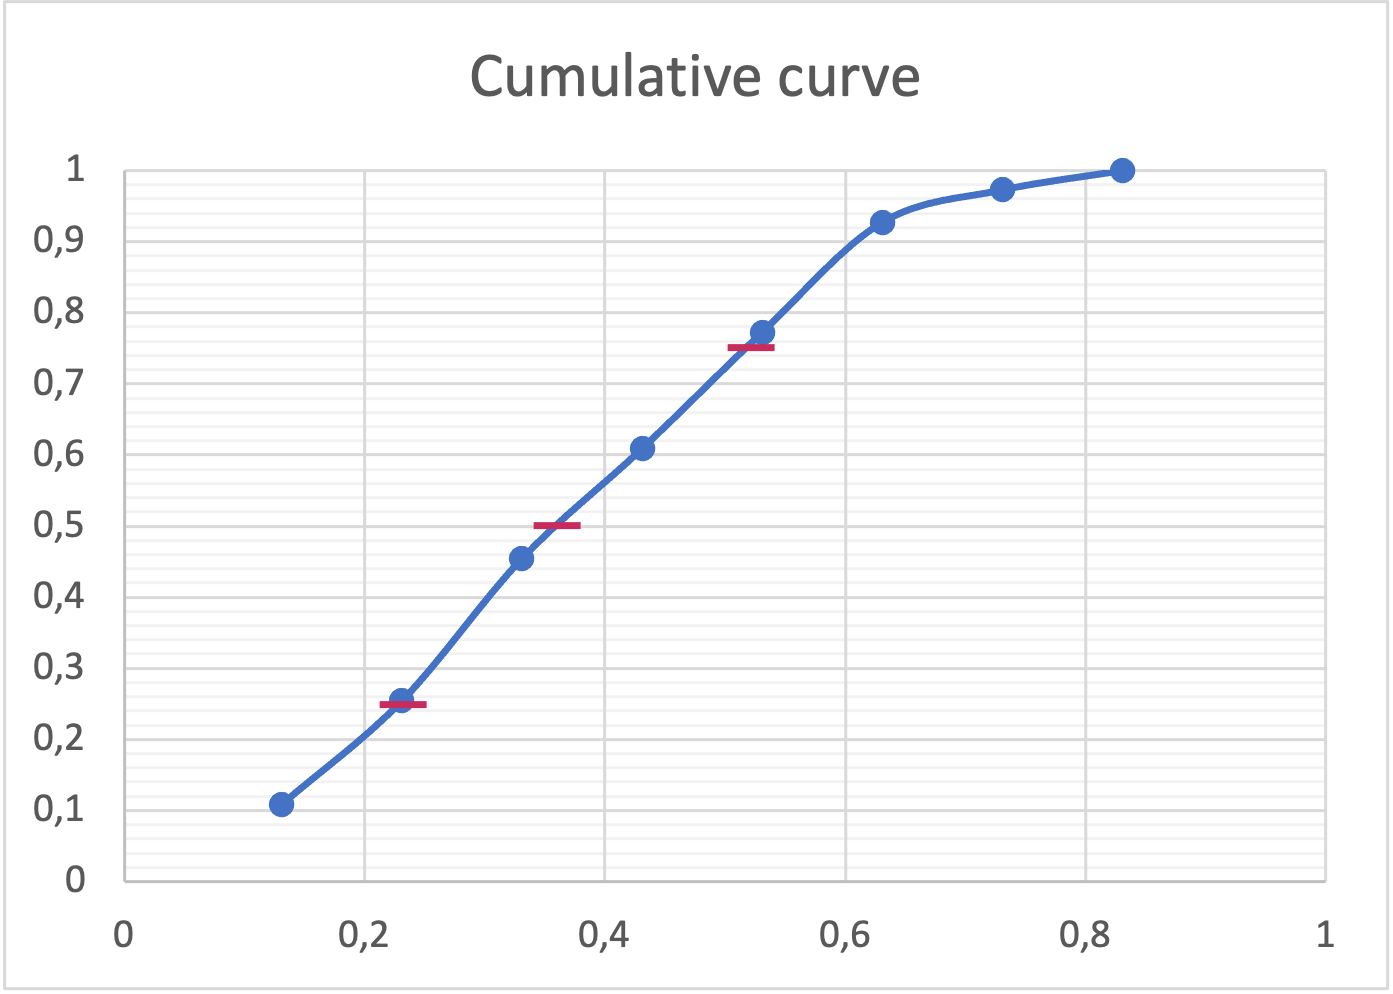
\includegraphics[width=\textwidth/2]{zvit1-1}

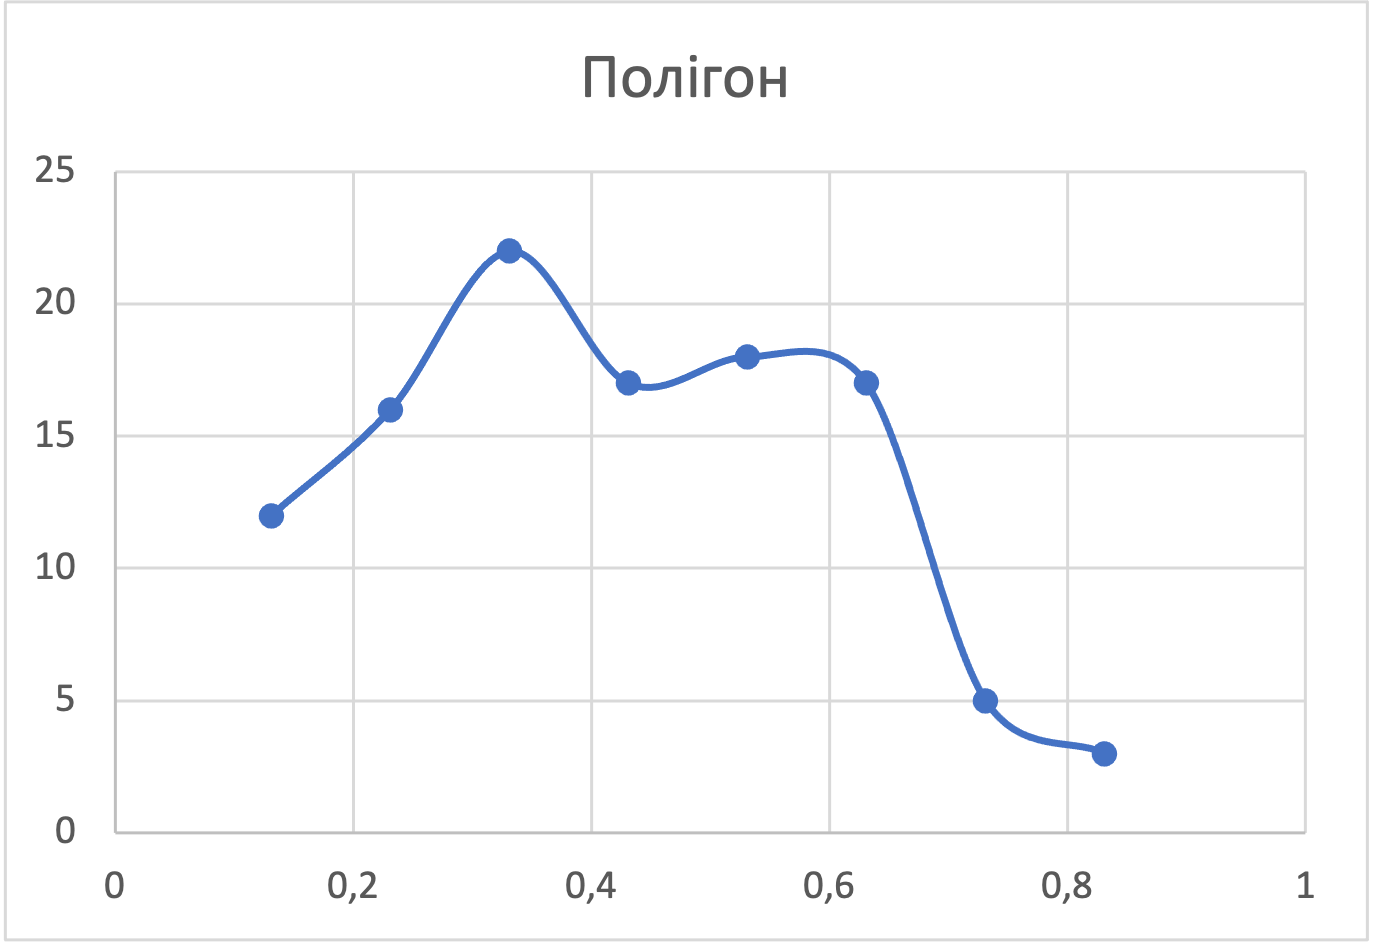
\includegraphics[width=\textwidth/2]{zvit1-2}

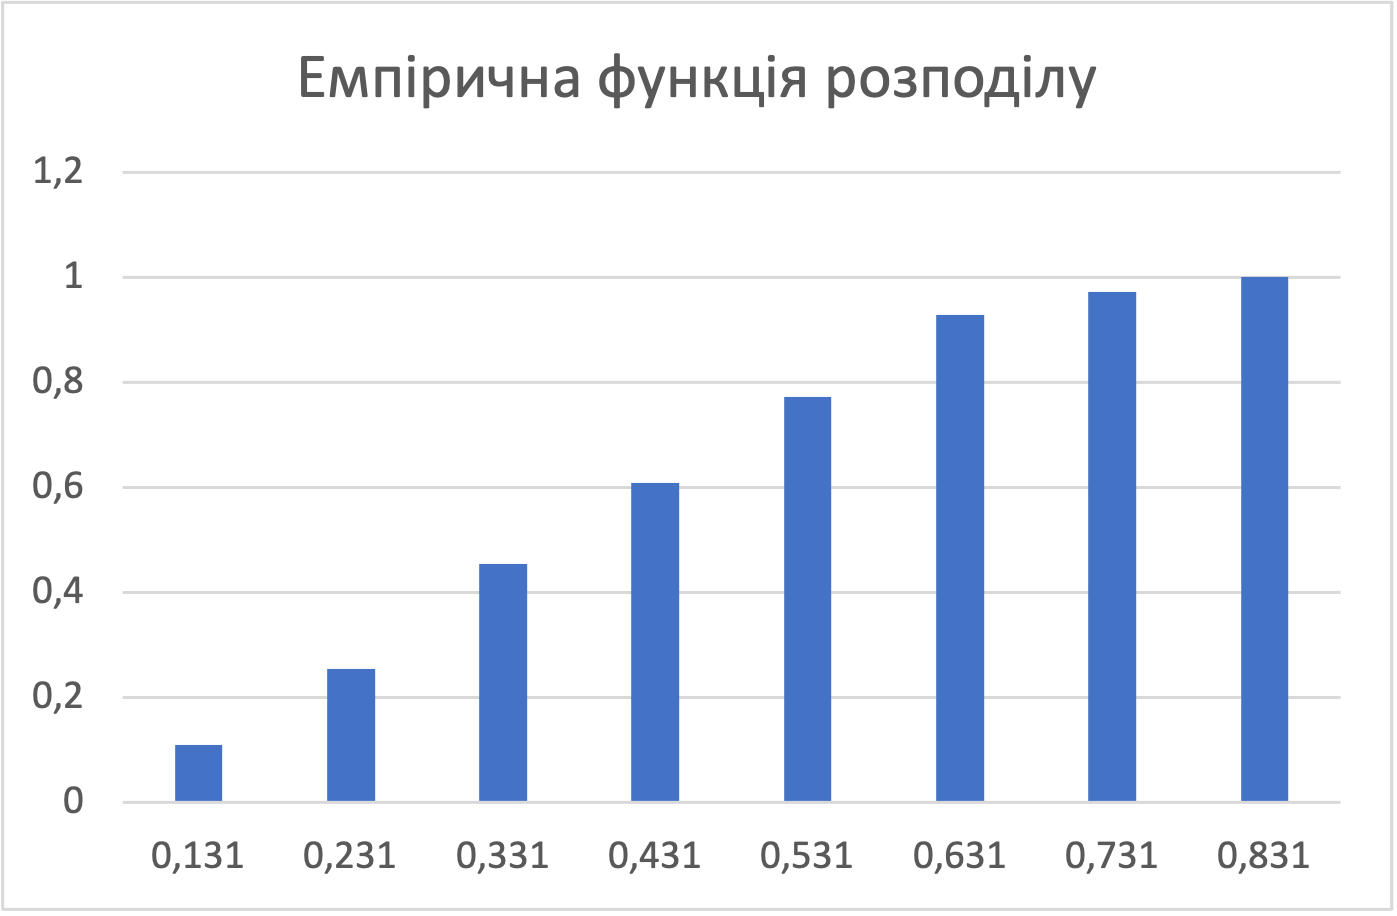
\includegraphics[width=\textwidth/2]{zvit1-3}

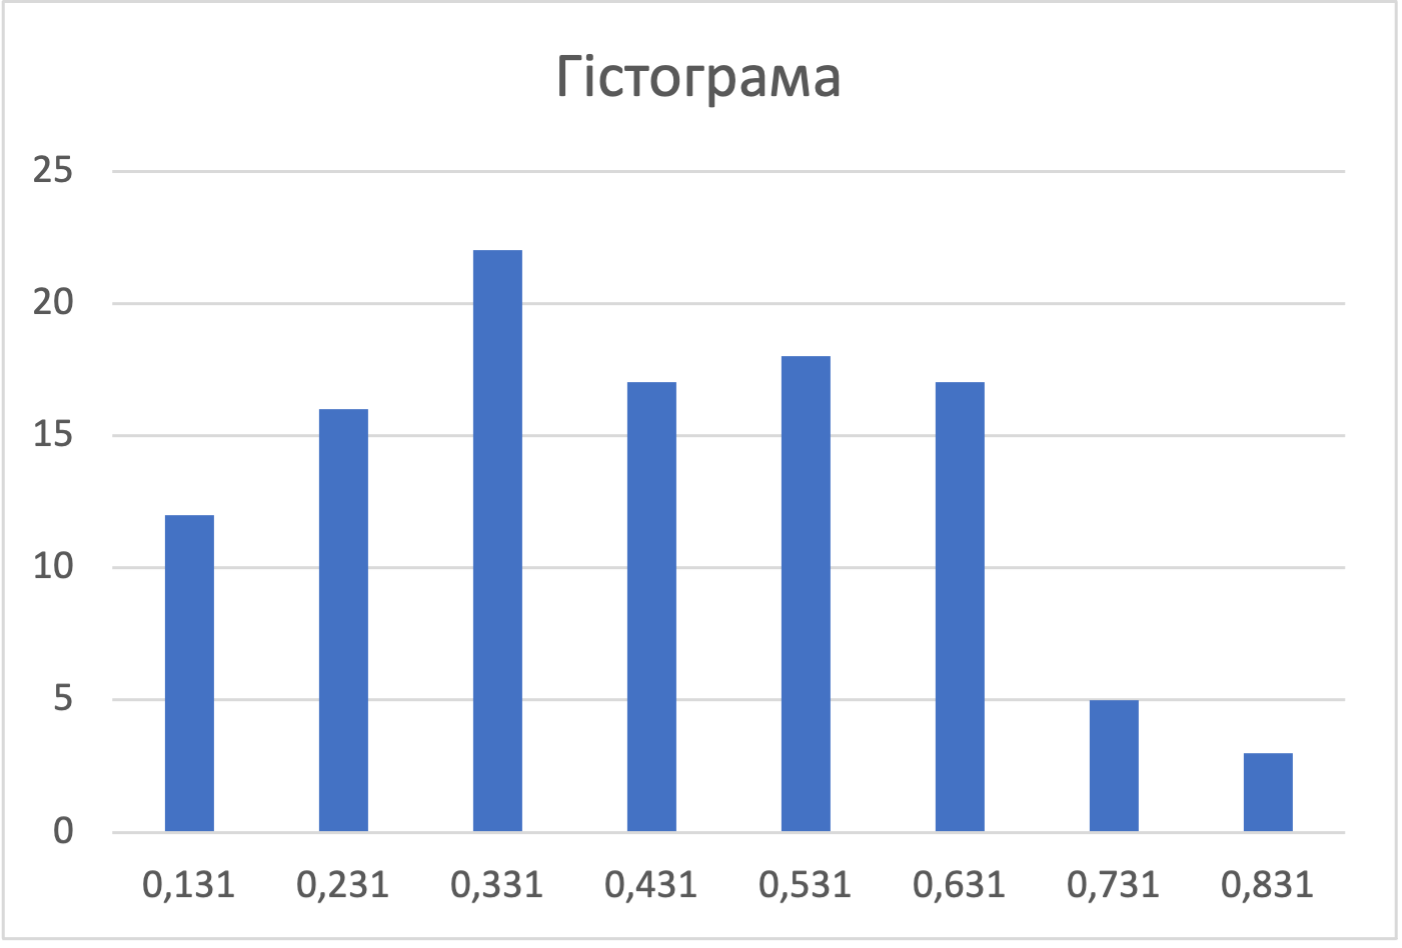
\includegraphics[width=\textwidth/2]{zvit1-4}

\section{Обчислити числові характеристики центральної тенденції та розкиду: вибіркове середнє, дисперсію, середньоквадратичне відхилення, моду, медіану, коефіцієнти асиметрії та ексцесу. Для обчислення застосувати табл.1 з прикладу 1.(2)}

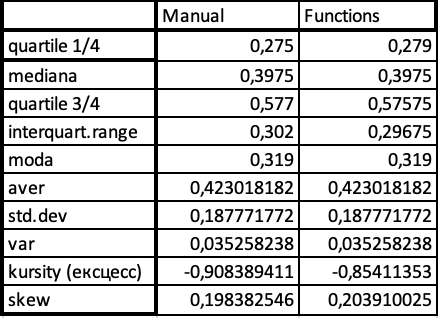
\includegraphics[width=\textwidth*2/3]{zvit1-n3}

\begin{description}
\item{-} Значення ексцесу < 3  характеризує плосковершинний розподіл.

\item{-} Коефіцієнт асиметрії є додатнім, тому це вказує на те, що розподіл має  правий хвіст. Але є майже симетричним оскільки значення наближається до 0.

\item{-} За припущенням тоді вибіркове середнє має бути більше за медіану.

$ aver = 0,423 >  0,3975 = mediana $, тому це твердження виконується

\end{description}

\section {Запропонувати своє бачення про природу даних і зробити висновок в предметній області. і скласти звіт. Завантажити на ДІСТЕДУ.(1)}

Дані варіанту №1 - можна припустити, що це система нарахування новорічної премії до заробітньої платні в компанії "Київтрансгаз", оскільки вони в межах від 0 до 1, невід'ємні. Для зручності можна перевести значення в відсотковий вигляд.

(або ще можна інтепретувати як знижки в супермаркеті на товари)

\subsection*{Висновок предметної області}

В отриманому прикладі розглядалось 110 значень нарахувань премії до заробітньої платні.

Мінімальне нарахування = 8,1\%

Максимальне нарахування = 84,3\%

Вибіркове середнє нарахування = $\sim 42,3\%$, медіана = $\sim 39,75\%$, що вказує на правий хвіст у розподілі.

Отримані дані було переведено в інтервальний статистичний ряд з інтервалами в 10\%. Найбільша кількість працівників мали нарахування в межах 28\% - 38\% = 22 людей.

Найменша кількість працівників мали нарахування в межах 68\% - 83\% = сумарно 8 людей (5 та 3 людей у відповідних інтервалах).

Інші нарахування були розподілені майже рівномірно по своїх інтервалах = від 12 до 18 людей.

Середнє квадратичне відхилення від середнього значення нарахування до 20\% = 18,8\%

Значення ексцесу -0,908 < 3  характеризує плосковершинний розподіл.

Коефіцієнт асиметрії є додатнім, тому це вказує на те, що розподіл має  правий хвіст. 

За припущенням тоді вибіркове середнє має бути більше за медіану.

$ aver = 0,423 >  0,3975 = mediana $, тому це твердження виконується.

 Це можна інтерпретувати як більшість нарахувань помірні з невеликою кількістю дуже вигідних для працівників (> 68,1\% нарахувань). 

Міжквартильний розмах = 57,7\% - 27,5\% = 30,2\% показує нарахування премії для людей, що потрапили в середні 50\% вибірки.

Найчастішим нарахуванням до заробітньої платні стало 31,9\% (мода)- тричі







\end{document}